%
% Reproducibility manuscript: describe results from relative
% alchemical free energy simulation done with various MD packages.
%
% arara: make
% arara: pdflatex
% arara: bibtex
% arara: pdflatex
% arara: pdflatex
% arara: clean: {files: [reprod.aux, reprod.bbl, reprod.blg, reprod.log, acs-reprod.bib]}
%


\documentclass[journal=jctcce,manuscript=article]{achemso}

\usepackage[T1]{fontenc}
\usepackage{graphicx}
\usepackage{amsmath,amssymb,mathrsfs}
\usepackage{booktabs}
\usepackage{multirow}
\usepackage{siunitx}
\usepackage{easy-todo}
\usepackage{footref}


\sisetup{
  separate-uncertainty = true
}

\renewcommand{\footnoterule}{}
\renewcommand{\vec}[1]{\mathbf{#1}}


\title{Reproducing Relative Alchemical Free Energies of Hydration
  (draft)}

\author{Hannes H. Loeffler}
\affiliation[Scientific Computing Department, STFC]{Science \&
  Technology Facilities Council, Daresbury, Warrington, WA4 4AD,
  United Kingdom}
\email{Hannes.Loeffler@stfc.ac.uk} \phone{+44 1925 603367}

\author{Stefano Bosisio}
\affiliation[University of Edinburgh]{EaStCHEM School of Chemistry,
  University of Edinburgh, David Brewster Road, Edinburgh EH9 3FJ, UK}

\author{Guilherme Duarte Ramos Matos}
\affiliation[University of California, Irvine]{Department of
  Chemistry, University of California, Irvine}

\author{Donghyuk Suh}
\affiliation[University of Chicago]{University of Chicago}

\author{Julien Michel}
\affiliation[University of Edinburgh]{EaStCHEM School of Chemistry,
  University of Edinburgh, David Brewster Road, Edinburgh EH9 3FJ, UK}

\author{David L. Mobley}
\affiliation[University of California, Irvine]{Departments of
  Pharmaceutical Sciences and Chemistry, University of California,
  Irvine}

\author{Benoit Roux}
\affiliation[University of Chicago]{University of Chicago}


\keywords{Free Energy, Hydration, Alchemical, Reproducibility, Automation}



\begin{document}

\begin{abstract}
  Alchemical free energy calculation is a very important branch of
  modern simulation techniques.  Contemporary Molecular Dynamics and
  Monte Carlo software such as AMBER, CHARMM, GROMACS and Sire/SOMD
  include support for the method.  Implementation details vary among
  those codes but users expect reliability and reproducibility i.e.\ a
  simulation must yield a comparable free energy within statistical
  bounds regardless of code used.  \emph{Relative} alchemical free
  energy simulation has been less well tested than its absolute
  counterpart in this context, however, relative transformations
  promise to be computationally and statistically more efficient.
  Here we present the results for relative hydration free energies
  (RAFE) for a set of small organic molecules and show that free
  energies can be satisfactorily reproduced with aforementioned codes.
  We will also recommend simulation protocols, setup procedures and
  analysis techniques.
\end{abstract}

\begin{tocentry}
  % \includegraphics[scale=1.0]{}
\end{tocentry}

\todo{Objectives:
 Do the relative free energy results produced across different
 softwares agree with each other? What if they don't?}

\todo{Objectives:
 Can we outline what should be a standard procedure to calculate
 relative free energies of hydration alchemically?}

\todo{Objectives:
 We want to emphasise that we aim at improving codes/protocols/practices and not highlight "bad" codes
}

\section{Introduction}
\label{sec:intro}

The free energy is a fundamental function of thermodynamics and
kinetics as it explains how processes in nature evolve.  The direction
that, say, a chemical reaction takes can be immediately determined
from the knowledge of the free energy difference of reactant and
product.  The free energy landscape of a given system, however, can be
very complicated and rugged such that barriers exist which impose
limits on how fast the process can take place.  It is therefore of
little surprise that the determination of this reversible work is of
utmost importance to all natural sciences e.g.\ for binding and
molecular association, solvation and solubility, protein folding and
stability, partition and transfer, and design and improvement of force
fields.

The calculation of free energies through
computers~\cite{hansen_practical_2014, doi:10.1021/jp102971x,
  Gallicchio201127, doi:10.1080/08927022.2015.1132317,
  doi:10.1146/annurev.matsci.32.111901.153708} has been particularly
attractive as it promises to circumvent limitations of experimental
approaches, processes can be understood at the molecular level and it
offers the potential of being more cost and time effective.  Thus, a
multitude of methods have been devised to make reversible work
estimates accessible through computation~\cite{hansen_practical_2014,
  doi:10.1021/jp102971x, Gallicchio201127,
  doi:10.1080/08927022.2015.1132317,
  doi:10.1146/annurev.matsci.32.111901.153708}.  However, the
reliability of estimates is still very much a matter of
concern~\cite{doi:10.1021/jp102971x, doi:10.1021/acs.jctc.5b00179}.
Roughly speaking, fast methods tend to be less accurate while more
accurate methods tend to be slow to compute.  Nevertheless, rigorous
methods are obligatory in obtaining accurate, precise and reliable
results, while less accurate methods can be used as an input filter
for more expensive approaches.

One such method is the so-called \emph{alchemical} free energy
approach whose theory is firmly rooted in statistical thermodynamics
and is argued to be the most accurate method in quantitative
prediction of free energies~\cite{Beveridge-citeulike:3789890,
  straatsma:92, doi:10.1021/cr00023a004, hansen_practical_2014}.  The
method has been applied in various forms for many decades now since
the early days of computer simulation~\cite{doi:10.1063/1.1671118,
  bennett_efficient_1976, doi:10.1063/1.432264, FS9821700055,
  Tembe1984281, doi:10.1063/1.449208}.  The method has gained renewed
attention in recent years --- concomitant with improvements in
computer hardware design --- both within the traditional equilibrium
framework~\cite{GILSON19971047, doi:10.1021/jp0217839,
  deng_computations_2009} but also increasingly being used in
non-equilibrium regimes~\cite{ytreberg_comparison_2006, JCC:JCC23804,
  doi:10.1021/ct500964e}.  The name comes from the nonphysical
intermediates that often need to be created to smoothly interpolate
between end states and because parts or all of a molecule may appear
or ``disappear'' in a transformation.  In the context of force field
methods the transformation takes place in parameter space i.e.\ the
force field's parameters determining strength and equilibrium of
interactions are varied by scaling.  This can be a particular
efficient approach as it does not require translocation in
configuration space.  For instance, the dissociation of a ligand from
a large biomolecule may involve many degrees of freedom while, at the
same time, it is generally unclear along which coordinates a
translocation simulation should take place.

Alchemical free energy simulations are constructed around the concept
of thermodynamic cycles.  As the free energy is a state function it
must always add up to zero within a closed cycle.  This also implies
that the reversible work can be computed arbitrarily along
conveniently chosen legs of the cycle.  E.g.\ in
Fig.~\ref{fig:thermocycle} the relative free energy of hydration can
be computed along the vertical legs, that is following the physical
process of moving a molecule from the gas phase to the liquid phase,
or along the horizontal legs in an nonphysical alchemical calculation.
As mentioned above, the latter may be computationally and
statistically more efficient.

\begin{figure}[ht]
  
\includegraphics[scale=1.0]{figures/thermocycle.pdf}
  \caption{The thermodynamic cycle to compute the relative free energy
    of hydration
    $\Delta\Delta G_{\mathrm{hydr}}=\Delta G_{\mathrm{sol}}-\Delta
    G_{\mathrm{vac}}=\Delta G'' - \Delta G'$.  The example is for the
    ethanol $\leftrightarrow$ methanol transformation.  Alchemical
    simulations can be performed along the non--physical horizontal
    legs while vertical legs illustrate the physical process (which is
    directly accessible through absolute alchemical free energy
    simulation, see [FreeSolv]).}
  \label{fig:thermocycle}
\end{figure}

Absolute (standard) alchemical free energy calculation has been a
particular focus of recent years~\cite{GILSON19971047,
  doi:10.1021/jp0217839, deng_computations_2009,
  ytreberg_comparison_2006, doi:10.1021/ct500964e}.  \emph{Absolute}
here really means that the equilibrium constant of a physical
reaction, e.g.\ binding and dissociation, can be calculated directly
by completely decoupling a whole molecule from its environment and the
term is mostly being used to discriminate against \emph{relative}
techniques (see below).  These schemes may require two simulations
along the parallel legs of a rectangular thermodynamic cycle but
approaches that produce the reversible work directly in one simulation
have been proposed too~\cite{doi:10.1063/1.3519057, C3FD00125C}.

Relative alchemical free energy (RAFE) calculations ``mutate'' one
molecule into another one.  This is most efficiently
achieved~\cite{doi:10.1021/j100056a020, Michel2010} by making use of
the single topology method~\cite{doi:10.1063/1.449208,
  doi:10.1021/j100056a020, doi:10.1021/jp981628n}.  Single topology
means that there is only one description of the molecule to be
mutated.  Thus, atom types are directly transformed into the new type,
typically by linearly scaling force field parameters.
Disappearing/appearing atoms are balanced with ``dummy'' atoms,
i.e. atoms that have no non--bonded interactions in the end state but
retain the bonded terms of the original atom.  AMBER is a special case
as it does not require the use of dummy atoms: the bonded terms of
atoms that do not exist in the end state will not contribute to the
free energy implying that contributions from dummy atoms perfectly
cancel in the thermodynamic cycle.  RAFEs are useful e.g.\ in ranking
which one of a set of small molecules binds strongest to a chosen
target.  This approach has recently gained more traction in the
context of relative free binding energies of
biomolecules~\cite{doi:10.1021/ja512751q}.

The single topology approach~\cite{doi:10.1021/j100056a020} requires a
certain similarity between the two mutated states.  This means
topological and structural similarity but also chemical similarity is
of importance e.g.\ chirality and binding modes where the relative
three dimensional arrangement in space must be taken care of.
Furthermore, ring breaking is technically
challenging~\cite{doi:10.1021/acs.jctc.6b00991} but it has also been
shown that this should be done only in certain
circumstances~\cite{doi:10.1021/acs.jcim.5b00057,
  doi:10.1021/jp994193s}.

When the two molecules are very dissimilar, the dual topology
method~\cite{doi:10.1021/j100056a020, doi:10.1021/jp981628n} can be
applied to compute relative free energies.  In this approach all atoms
in the end states are duplicated and thus both sets are present at all
times but don't interact with each other.  Only non--bonded
interactions need to be scaled such that the disappearing end state
corresponds to an ideal gas molecule~\cite{doi:10.1021/jp981628n}.
This, however, comes with additional complications as two independent
molecules can drift apart and so suffer from the ``wandering'' ligand
problem as in absolute transformations\cite{GILSON19971047,
  doi:10.1021/jp0217839, deng_computations_2009}.  Topolological
similarity can only be exploited when the charges of the common core
are explicitly made equivalent~\cite{doi:10.1021/acs.jctc.5b00179}.
This approach, however, shifts all the chemical variability
exclusively to the dummy atoms and is thus of only limited use.

Technically, a dual topology calculation is the same as two absolute
calculations run simultaneously in opposite directions.  It has been
shown though that with the introduction of special restraints or
constraints this can be a viable option~\cite{doi:10.1021/ct700081t,
  rocklin_separated_2013}.  A covalent link, e.g.\ as in side--chain
mutation simulations, provides a natural restraint such that dual
topology simulations can be applied without further problems.  Modern
MD software e.g.\ AMBER~\cite{case_amber_2005},
CHARMM~\cite{JCC:JCC21287}, GROMACS~\cite{Abraham201519},
GROMOS~\cite{doi:10.1021/jp984217f} and Sire/SOMD~\cite{Sire-2016,
  doi:10.1021/ct300857j} offer a hybrid single/dual topology approach
i.e.\ the user can specify which part of a perturbed group should be
handled by which method~\cite{doi:10.1021/jp994193s}.  The perturbed
group comprises of all atoms that differ in at least one force field
parameter between the end states.

As alluded to above, reliability is a principal matter of concern.  In
particular, we need to ensure reproducibility of free energy results
among computer codes.  To the best of our knowledge this has not been
systematically tested yet for a set of different MD packages.  Given a
predefined force field and run--time parameters we should be able to
obtain comparable free energy results within statistical convergence
limits.  In practice, we have the problem, however, that the methods
and algorithms used in MD programs are not always present in all
packages or are the same, like pressure and temperature scaling,
integrators, etc.  Nevertheless, the reversible work computed with any
simulation software should be expected to be reproducible.  Modern MD
packages support a wide range of force fields and methods such that
these packages are replaceable with each other to an ever increasing
extent and the choice of the right package for the user becomes less
and less a matter of technical restrictions.

In this work we present the results of relative hydration free
energies of a set of small organic molecules (see
Fig.~\ref{fig:cycles}).  Solvation free energies have a wide range of
uses and various methods exist to compute
them~\cite{Skyner:2015:PCCP}.  They are also needed to calculate
binding free energies where the simulation in solution (see
Fig.~\ref{fig:thermocycle}) is combined with a mutation of the
molecule bound to a partner, and other important physical
properties~\cite{Skyner:2015:PCCP}.  A large database of hydration
free energies computed from AFE simulation, FreeSolve, has been
presented recently (cite). Here, we are interested in the
reproducibility of RAFE with the simulation programs AMBER, CHARMM,
GROMACS and Sire/SOMD.  We will discuss the reversible work results
obtined with these packages as well as making recommendations
regarding simulation protocols, setup procedures and analysis
techniques.


\section{Methods}
\label{sec:methods}

\subsection{Alchemical Free Energy Implementations}
\label{sec:afe_impl}

We begin by working out the differences in the alchemical free energy
implementations of the four MD codes AMBER, CHARMM, GROMACS and
Sire/SOMD.  One key difference is the softcore
functions~\cite{beutler_avoiding_1994,
  zacharias_separationshifted_1994} used in each code as summarised in
the SI.  Softcore functions are used to avoid numerical and thus
stability problems of the conventional van der Waals and Coulombic
potentials~\cite{steinbrecher_nonlinear_2007} as they have
singularities at zero distance (vertical asymptotes).  Direct scaling
of these potentials causes the functions to increasingly behave like
hard--sphere potentials as $\lambda\rightarrow 0$.  This implies a
higher probability of other atoms to penetrate into the highly
repulsive short--range portion of the potential which can lead to
strongly fluctuating forces/energies and to severe instabilities in
the integrator.

Other differences are whether the code scales individual (force field)
parameters and/or the total energy~\cite{doi:10.1021/jp981628n}, or if
the code allows constraints for bonds with changing bond lengths.
These and other details will be outlined below.  The perturbed group
comprises of all atoms that need to be transformed, i.e.\ any atom
that differs in at least one force field parameter in the other end
state.

\paragraph{AMBER} This code is strictly dual topology and all terms
are energy--scaled.  The code allows, however, to map atoms in a
single topology fashion and computes the forces appropriately
(linearly) scaled for each atom in the pair.  The perturbed group must
be entirely duplicated i.e.\ for sander this means two topology files
with one end state each, or for pmemd both end states in one topology
file.  The softcore potential applies to dummy atoms only but which
can be arbitrarily chosen by the user.  Explicit dummy atoms are not
needed as the code will only compute bonded contributions for ``real''
atoms thus ignores bonded energies involving dummy atoms.  The code
cannot handle constraints of changing bond lengths in the perturbed
group.  There is only on global $\lambda$ for parameter
transformation.  Separated protocols (see below) must be emulated
through careful construction of topology files.

\paragraph{CHARMM} The PERT module duplicates the topology similar to
sander but requires explicit dummy atoms.  All terms are
energy--scaled.  The PSSP softcore potential is applied to \emph{all}
atoms in the perturbed group (see SI).  The code can handle
constraints of changing bond lengths in the perturbed group but this
may cause wrong results with PSSP softcores (Stefan Boresch, private
communication).  There is only one global $\lambda$ for parameter
transformation, however, the scripting facilities allow run time
modification of topologies e.g.\ by setting charges or vdW parameters
to arbitrary values.

\paragraph{Gromacs} This code uses a single topology description.
Bonded terms are strictly parameter--scaled which requires proper
balancing of multi--term dihedrals.  Non--bonded terms are
energy--scaled.  The softcore potential applies to dummy atoms only
which are determined if atoms have zero vdW parameters.  The code
allows constraints of changing bond lengths in the perturbed group but
this can lead to instabilities and wrong results (Michael Shirts,
private communication).  There are separate $\lambda$s for vdW,
Coulomb and bonded parameters (and some other).

\paragraph{Sire/SOMD} This code uses a single topology description.
The final state is constructed at run time from the initial state with
a ``patch'' (list of force field parameters to be modified).  Bond and
angle terms are parameter--scaled while all other terms are
energy--scaled.  The softcore potential applies to dummy atoms only.
The code cannot handle constraints of changing bond lengths in the
perturbed group.  There is only one global $\lambda$ for parameter
scaling.  Separated protocols (see below) must be emulated through
careful construction of the patch file.  Sire/SOMD is
Sire~\cite{Sire-2016} employing OpenMM~\cite{doi:10.1021/ct300857j}
for MD simulation.

\subsection{RAFE Setup}
\label{sec:rafe_setup}

The setup for all relative free energy simulations has been carried
out with the tool FESetup~\cite{loeffler_fesetup:_2015} in version
1.2.  FESetup is a perturbed topology writer for AMBER, CHARMM,
GROMACS, Sire/SOMD and also NAMD~\cite{JCC:JCC20289} (within the
limits of the dual topology approach).  The tool makes use of a
maximum common substructure search algorithm to automatically compute
atoms that can be mapped i.e.\ atoms that have a direct relationship
to an equivalent atom in the other state.  This means atom type to
atom type conversion and the only current limit is that rings are
required to be preserved~\cite{doi:10.1021/acs.jcim.5b00057}.  In this
way we achieve a maximal single topology description: any atom that
does not match will be made a dummy atom.  FESetup allows
equilibration of the solvated simulation systems and ensures that
``forward'' and ``backward'' simulations will have the same amount of
total atoms.  The tool creates all input files with control
parameters, topologies and coordinates as required for RAFE
simulations.  Full details on FESetup can be found in
Ref.~\citenum{loeffler_fesetup:_2015}.

Figure~\ref{fig:cycles} shows all 18 transformation considered in this
study including ``forward'' and ``backward'' mutations.  RAFE
simulations are principally fully symmetric i.e.\ they do not have a
directionality with respect to the coupling (order) parameter
$\lambda$.  Performing simulations in either direction, however, is
applied here as a test for possible discrepancies.

\begin{figure}[ht]
  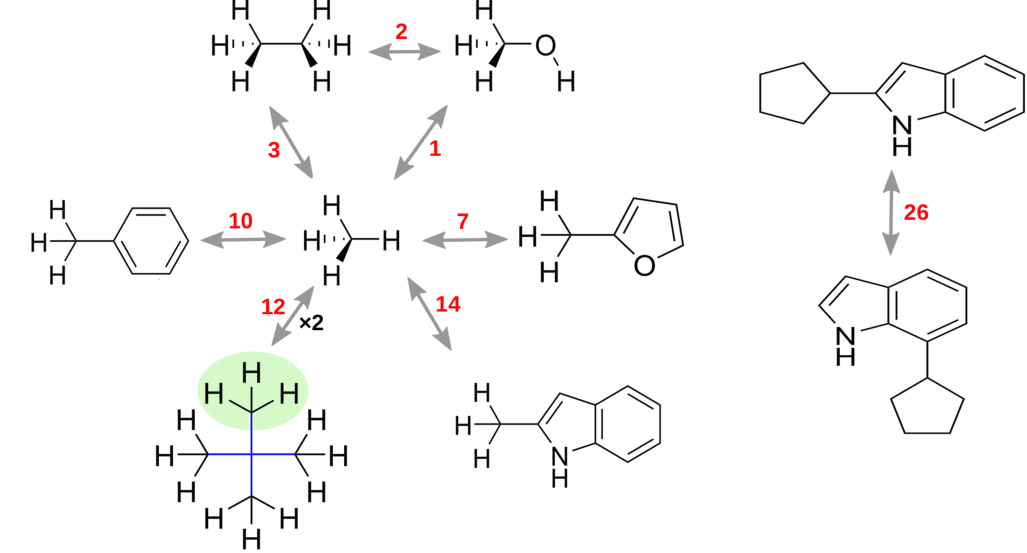
\includegraphics[scale=1.0]{figures/cycles.pdf}
  \caption{The thermodynamic cycles considered in this study.  To
    compute the free energy of hydration all pair--wise
    transformations have to be carried out once in solution and once
    in vacuum.  Green and blue colours in neopentane show two
    alternative mappings for methane.  The numbers in red denote the
    number of dummy atoms.}
  \label{fig:cycles}
\end{figure}

The ethane $\rightarrow$ methanol transformation is traditionally
regarded as a standard test for RAFE
simulations~\cite{doi:10.1063/1.449208, doi:10.1021/jp981629f}.  The
other transformations are centred around mutations from and to
methane.  The 2--cyclopentanylindole to 7--cyclopentanylindole
transformation has been added to include both deletion as well as
insertion of sub--parts of the perturbed group in one simulation.  For
neopentane $\rightarrow$ methane we point out that there are two
alternative mappings possible, see Figure~\ref{fig:cycles}.  One in
which methane is mapped with a terminal methyl (green) and the other
one where the methane carbon is mapped with the central carbon in
neopentane (blue).  Results from both mutations will be shown and
discussed.


\subsection{RAFE Simulation Protocols}
\label{sec:rafe_protocols}

One of the major concerns in a reproducibility study is to ensure
consistency in the applied protocols.  This is complicated by the fact
that MD software employs a wide range of methods and algorithms that
may not be available in other MD software.  For example, pressure and
temperature scaling, integrators and other algorithms can be very
different.  It is also unclear if and how implementation details can
affect results, in particular see discussion in
subsection~\ref{sec:afe_impl} of alchemical free energy
implementations.

In this study we look at a set of simple organic molecules (see
Figure~\ref{fig:cycles}).  As the focus here is on probing for
reproducibility among various MD packages, we chose fairly small,
rigid and neutral molecules to keep problems with sampling low, and
avoid difficulties with charged
particles~\cite{rocklin_calculating_2013, JCC:JCC1050}.  The force
field was chosen to be GAFF~\cite{wang_development_2004} in version
1.8 utilising AM1/BCC charges~\cite{jakalian_fast_2000,
  jakalian_fast_2002} for the solute and
TIP3P~\cite{jorgensen_comparison_1983-1} for the solvent.  The quality
of free energies of various small molecule force fields has been shown
elsewhere, see e.g. Refs.~\citenum{doi:10.1021/ct300203w,Hu2016}.

While the MD packages principally allow a ``one--step'' transformation
that is both van der Waals and Coulombic contributions can vary
simultaneously, it can be(is? ref?) more efficient to carry out a
separated protocol.  In such a protocol the charges are transformed
linearly between the end states followed by a mutation of the van der
Waals parameters using a softcore
potential~\cite{beutler_avoiding_1994,
  zacharias_separationshifted_1994} (see SI for details) on the vdW
term only.  It is important to note that in the separated protocol
charges have to be switched off before vdW parameters (and vice versa
for the transformation in opposite direction) to avoid collapse of
other molecules e.g. solvents onto a ``naked'' charge, see SI.  This
has consequences for setting up simulations as discussed (somewhere
else).

All simulations were started from the simulation box pre--equilibrated with
FESetup~\cite{loeffler_fesetup:_2015}.  It should be noted, however, that in
constructing the system steric overlaps between the solute and the solvent can
happen.  This is because the number of atoms are always chosen to be the same
for forward and backward setups by using the larger box of the two.  Thus, in
transformation from a smaller to a larger solute water molecules may be in
close distance.  The simulations were run at \SI{298.15}{K} and \SI{1.0}{bar}.

\paragraph{AMBER} The starting coordinates were usually taken from the
starting state as taken from the setup step.  In some cases it was
necessary though to use coordinates from a nearby $\lambda$ state.
Water hydrogens (TIP3P) were constraint with SHAKE.  None of the atoms
in the perturbed group were constraint and so the time step was set to
\SI{1}{fs} (see Sire protocol below for an alternative approach).
Temperature was controlled through a Langevin thermostat and pressure
through a Monte Carlo barostat.

\paragraph{Sire/SOMD} All simulations were carried out with
Sire/OpenMM 6.3 (revision 16.1).  Each alchemical transformation was
divided into 17 evenly spaced windows and simulated for \SI{2}{ns}
both in water an vacuum phase. A velocity-Verlet integrator was
employed with \SI{2}{fs} timestep, constraining all the hydrogen bonds
not alchemically transformed (unperturbed H protocol). An atom--based
Barker--Watts reaction field~\cite{doi:10.1080/00268977300102101} with
a dielectric constant of \num{82.0} was employed for water phase
simulations. A cutoff of \SI{12}{\angstrom} was set for non-bonded
interactions and periodic boundary conditions were imposed.
Temperature control was achieved with the Andersen
thermostat~\cite{doi:10.1063/1.439486} with a coupling constant of
\SI{10}{ps^{-1}}.  A Monte Carlo barostat assured pressure control,
attempting isotropic box edge scaling every 25 time steps. At each
$\lambda$ window all bond, angle and dihedral energy terms were
scaled, differently (how?) from Gromacs and Amber.  For each vacuum
simulation a free energy correction term $G_{\mathrm{FUNC}}$ was
evaluated to treat intramolecular Coulombic interactions consistently
between water and vacuum legs of the thermodynamic cycle, as explained
in~\cite{Bosisio2016} (some details here?).


\subsection{Analysis}
\label{sec:analysis}

Various estimators have been proposed to obtain the free energy.
Early work by Kirkwood~\cite{kirkwood_statistical_1935} expresses the
free energy as an ensemble average of the derivative of the
Hamiltonian with respect to the coupling parameter $\lambda$.  The
method is now known as Thermodynamic Integration (TI).  Zwanzig
devised the exponential formula~\cite{zwanzig_high-temperature_1954}
(EXP), also known as Free Energy Perturbation (FEP) or thermodynamic
perturbation (TP), which calculates the free energy from the
exponential average of the energy difference of the end states.  The
energy difference is computed with the configuration of one end state
being used for both end states assuming that this configuration is
representative for either state.  As the phase--space overlap needs to
be sufficiently large~\cite{wu_phase-space_2005,
  wu_phase-space_2005-1} the EXP approach typically needs
intermediates, controlled by $\lambda$.  However, it has been shown
that EXP has an asymmetric bias depending on the directionality of
$\lambda$~\cite{wu_asymmetric_2004} and that the Bennett Acceptance
Ratio (BAR) method~\cite{bennett_efficient_1976} is considerably more
effective in obtaining an accurate result~\cite{lu_appropriate_2003}.
BAR is a generalisation of EXP by making explicit use of the
``forward'' ($\lambda_i \rightarrow \lambda_{i+1}$) and ``backward''
($\lambda_{i+1} \rightarrow \lambda_i$) estimates.  Later is has been
demonstrated that this can be effectively extended to incorporating
more than just the immediate $\lambda$ neighbour and, in fact, all
other $\lambda$s.  This approach has been called multi--state BAR
(MBAR)~\cite{shirts_statistically_2008-1} method.  MBAR has been shown
to have the lowest variance of any known
estimator~\cite{shirts_statistically_2008}.

In this work we primarily focus on TI as this is supported by all MD
packages ``out--of--the--box''.  Equation~\ref{eq:ti} computes the free energy as
\begin{equation}\label{eq:ti}
	\Delta G = \int_{\lambda=0}^{\lambda=1}
	\left\langle \frac{\mathscr{H}(\vec{q},\vec{p};\lambda)}{\partial\lambda}\right\rangle_\lambda d\lambda
\end{equation}
where $\mathscr{H}(\vec{q},\vec{p};\lambda)$ is the Hamiltonian as a function of the coordinate vectors $\vec{q}$ and the momentum vectors $\vec{p}$, and parametric dependence on the coupling parameter $\lambda$.  The angle brackets denote the ensemble average of the gradient of the Hamiltonian with respect to $\lambda$ at a given $\lambda$ value.  An AFE simulation is typically carried out in a series of equilibrium simulations at discrete values of $\lambda$ but the gradient can also be evaluated with a continuously varying coupling parameter as a function of the simulation time.  The free energy is finally computed through a suitable numerical integration method.

Results from additional estimators
will be given where available.  We have used the alchemical analysis
tool~\cite{klimovich_guidelines_2015} for all free energies.  This
tools provides various estimators such as TI, TI with cubic splines,
BAR and MBAR.  All data can be sub--sampled to eliminate correlated
data.

All RAFE simulations where run in triplicate in forward as well as
backward direction so in total 6 simulations per mutation pairs.  The
final hydration free energy $\Delta\Delta G_{\mathrm{hydr}}$ was
computed as average of each direction.  For comparison we have also
calculated the absolute (standard) hydration free energies for all
molecules in Figure~~\ref{fig:cycles}).

To estimate the reliability and convergence of the results, the
standard error of the mean (SEM) has been calculated.  The SEM is
defined as

\begin{equation}
  \label{eq:sem}
  \mathrm{err}(\Delta\Delta G_{\mathrm{hydr}}) = \frac{\sigma}{\sqrt{n}}
\end{equation}

where $\sigma$ is the sample standard deviation and $n$ is the size of
the sample.  The SEM for component free energies is combined as

\begin{equation}
  \label{eq:sem-comb}
  \mathrm{err}(\mathrm{combined}) = \sqrt{\sum_i \sigma_i^2}.
\end{equation}

which is appropriate if the property to be computed is a sum of
contributions.


\section{Results}
\label{sec:results}

\todo{what protocols did not work}

\todo{look into Fennell, C. J.; Wymer, K. L.; Mobley, D. L. Journal of
 Physical Chemistry B 2014, 118, 6438-6446 for errors in hydroxyl
 compounds (absolute transformations!) and Mobley, D. L.; Bayly, C. I.; Cooper, M. D.; Dill, K. A. The Journal of Physical Chemistry B 2009, 113, 4533-4537 for other functional groups.}

\todo{problems:
    e.g. methane~2-methylindole: needed to use restart file from
    l=0.95 to start simulation at l=1.0.
}

\subsection{AMBER}
\label{sec:amber-results}

\todo{2-cylco to 7-cyclo: report results, partial vs complete de/recharging}

Using AMBER for RAFE simulations has revealed several problems with
the implementation.  Some bugs could be idendified and have been fixed
by the developers e.g. energy minimisation in sander led to diverged
coordinates for mapped atoms which is, however, a necessary condition
for a single topology description.  Other issues are that vacuum
simulation have to be carried out separately with the sander program
because pmemd cannot handle AFE simulations in vacuum at the moment.  This will, however, be rectified in future versions (Ross Walker, private communication).  A disadvantage of sander is that it cannot be used to simulate the $\lambda$ end points~\cite{doi:10.1021/ct400340s} such that the TI gradients need to be extrapolated (minimum and maximum allowed $\lambda$s are 0.005 and 0.995).  Also, sander considers the whole system as the perturbed
region while pmemd restricts this to the user chosen TI region.  This
has obvious implications for performance~\cite{doi:10.1021/ct400340s}.

We also found that, in contrast to the other three codes, AMBER cannot
correctly reproduce relative free energies in a 1--step protocol i.e.\
when all force field parameters are scaled simultaneously (see SI for
details).  The separated RAFE protocol and absolute free energies,
however, are very close to the other MD packages.

End point geometries also appear to be an issue with AMBER simulations
in both solution and vacuum as most obvious in the neopentane to
methane (central mapping) test case.  As detailed in the SI the
methane end state shows too long distances between the carbon and the
four attached hydrogens of approximately \SI{1.23}{\angstrom}.  This
value is about \SI{1.12}{\angstrom} for terminal dummy atoms but still
higher than the expected, on average, \SI{1.09}{\angstrom}.

We also compare free energies obtained from the no--explicit dummy approach in AMBER with results form explicit dummy atom simulations and resuls from absolute transformation.  Table~\ref{tab:amber-comp} lists the free energies for these three approaches together with the SEM.
\begin{table}[]
  \begin{minipage}{\linewidth}
  \caption{Comparing AMBER results for simulations with implicit and explicit dummy atoms, and results from absolute transformation.}\label{tab:amber-comp}
  \makebox[\textwidth][c]{
  \begin{tabular}{llrrrrrr}
    \toprule
    &                & \multicolumn{2}{c}{implicit} & \multicolumn{2}{c}{explicit} & \multicolumn{2}{c}{absolute} \\
    \multicolumn{2}{l}{transformation}          & $\Delta\Delta G$  & SEM               & $\Delta\Delta G$    & SEM &  $\Delta G$\footnote{sign for the forward transformation.} & SEM \\
    \midrule
ethane         & methane        & 0.021    & 0.014 & -0.127 & 0.016 & \multirow{2}{*}{-0.022} & \multirow{2}{*}{0.012} \\
methane        & ethane         & 0.001    & 0.025 & 0.187  & 0.028 & &        \\
methanol       & methane        & 6.189    & 0.014 & 6.200  & 0.017 & \multirow{2}{*}{6.201} & \multirow{2}{*}{0.012} \\
methane        & methanol       & -6.195   & 0.029 & -6.145 & 0.013 & &         \\
ethane         & methanol       & -6.200   & 0.012 & -6.268 & 0.009 & \multirow{2}{*}{-6.223} & \multirow{2}{*}{0.014} \\
methanol       & ethane         & 6.196    & 0.014 & 6.252  & 0.011 & &         \\
toluene        & methane        & 3.240    & 0.020 & 3.386  & 0.021 & \multirow{2}{*}{3.193} & \multirow{2}{*}{0.014} \\
methane        & toluene        & -3.422   & 0.025 & -3.523 & 0.033 & &         \\
neopentane\footnote{\label{foot:cent}central mapping.} & methane & 0.315    & 0.038 & -0.027 & 0.057 & \multirow{4}{*}{-0.132} & \multirow{4}{*}{0.016} \\
methane\footref{foot:cent}        & neopentane     & -0.250   & 0.032 & 0.071  & 0.026 & & \\
neopentane\footnote{\label{foot:term}terminal mapping.}    & methane        & -0.132   & 0.012 & -0.118 & 0.015 & & \\
methane\footref{foot:term}        & neopentane    & 0.125    & 0.031 & 0.123  & 0.034 & & \\
2-methylfuran  & methane        & 3.089    & 0.014 & 3.102  & 0.009 & \multirow{2}{*}{2.964} & \multirow{2}{*}{0.023} \\
methane        & 2-methyfuran   & -3.100   & 0.032 & -3.147 & 0.033 & &         \\
2-methylindole & methane        & 8.778    & 0.025 & 8.777  & 0.041 & \multirow{2}{*}{8.717} &\multirow{2}{*}{0.009} \\
methane        & 2-methylindole & -9.138   & 0.022 & -9.130 & 0.034 & \\
    \bottomrule
  \end{tabular}
}
  \end{minipage}
\end{table}

In general, the free energies computed with each approach are in good agreement with each other and with the results of the other MD packages.  There are, however, a few notable deviations.  In the neopentane to methane case with the central mapping the difference with the terminal mapping is about \SI{0.4}{kcal.mol^{-1}}.  The terminal mapping and the results from the explicit dummy simulations are, however, consistent with the absolute transformations.  We also observe a systematic deviation between forward and backward transformations in the 2--methylindole and toluene vacuum simulations.  This discrepancy is evident for every $\lambda$ step of the vdW plus bonded transformation with both implicit and explicit dummy atoms.

\subsection{CHARMM}
\label{sec:charmm-results}

\todo{bug in TI gradient accumulation in parallel runs (does not affect
	serial?, does not affect EXP)}

\todo{cannot handle LRC: test with larger cutoffs and/or LRC correction
	with arbitrary, single structure}


\subsection{GROMACS}
\label{sec:gromacs-results}


\subsection{Sire/SOMD}
\label{sec:somd-results}

Results for Sire relative free energy calculations are shown in (FIG OR TABLE
TO BE DECIDED. Plot for MUD for each package?) good/bad agreement, final MUD =
?)

To achieve reproducibility the role of constraints was extremely
influential.  Fig.\ X shows the comparison between relative hydration
free energies computed by using different constraint schemes during
the simulation. When all bonds of the ligand are constraint a
systematic offset with respect to the other constraints with a MUD =
\SI{0.38}{kcal.mol^{-1}} was observed with respect to the no
constraint case and MUD = \SI{0.36}{kcal.mol^{-1}} compared to the
unperturbed H protocol (see section~\ref{sec:rafe_protocols}).
Furthermore, analysing these simulations with Gromacs and Amber all
bond constraints bring a MUD = \SI{1.2}{kcal.mol^{-1}}. The main
problem, for all bond constraints in RAFE calculations in Sire, is the
missing overlap between the potential energy functions between each
$\lambda$--step.  Further discrepancies appear when different
mappings and all bonds are constraint as Fig.\ X shows.

Referring to Fig.\ X, transforming neopentane to methane (centrally
mapped) shows a $\Delta\Delta G_{\mathrm{hyd}}$ of \SI{2.04 +-
  0.01}{kcal.mol^{-1}}, while for the backward transformation
$\Delta\Delta G_{\mathrm{hyd}}$ = \SI{-2.10 +- 0.01}{kcal.mol^{-1}},
which highly overestimates the free energy compared to Gromacs and
Amber (REFER TO TAB). Unexpectedly, simulation of neopentane to
methane (terminally mapped) shows a $\Delta\Delta G_{\mathrm{hyd}}$ =
\SI{0.59 +- 0.01}{kcal.mol^{-1}} and $\Delta\Delta G_{\mathrm{hyd}}$ =
\SI{-0.48 +- 0.01}{kcal.mol^{-1}} for the reverse transformation.  As
the free energy must be independent of the chosen path the discrepancy
highlights a problem with using constraints on transformed atoms.  The
solution adopted to achieve reproducibility in Sire is to rely on the
unperturbed H protocol.  These constraints allow a timestep of 2\,fs
with a MUD of \SI{0.30 +- 0.01}{kcal.mol^{-1}} with respect to Gromacs
and Amber.

To test the quality of relative free energies of hydration,
$\Delta\Delta G$ were estimated also with absolute free energy
calculations.  By computing the difference between absolute hydration
of methane and all the other molecule, the relative free energy of
hydration was computed.  Fig.\ X demonstrates the reliability of the
unperturbed H protocol through consistency between relative and
absolute simulations.  Furthermore, all the calculations can be
performed in one step, differently (how?) from Amber and Gromacs.
(EXPLAIN EXACTLY WHY)


\section{Discussion}
\label{sec:discuss}

\todo{recommended protocols}

\todo{protocols to avoid}

\todo{lessons learned}

\todo{2-cyclopentanylindole to 7-cyclopentanylindole: better to go through intermediates?}

\todo{
 AMBER: IMPORTANT: look at noshakemask, timask no SHAKE on real
 atoms? (symmetry) tishake=1 removes SHAKE to softcore atoms, ntf=1
 required for softcores because SHAKE \emph{may} be removed for some bonds;
 check if SHAKE is handled in for perturbed atoms end distances in
 crowded situation.
}

\todo{
 what do we need to progress the field e.g. automation to make things
 easy but also consistent and thus more reproducible (FESetup also
 for reproducibility) GPU: Gromacs, SOMD but not AMBER (yet) and
 CHARMM
}

\todo{
 developer notes: constraints, both appearing/disappearing
 atoms lambda paths for AMBER (relative), absolute: crgmask requires
 vacuum corr
}

\todo{further investigation required: binding RAFEs?}


\listoftodos


\begin{acknowledgement}
  HHL is supported through an EPSRC provided SLA, funding the core
  support of CCPBioSim.  CCPBioSim is the Collaborative Computational
  Project for Biomolecular Simulation funded by EPSRC grants
  EP/J010588/1 and EP/M022609/1.  JM is supported by a Royal Society
  University Research Fellowship.  The research leading to these
  results has received funding from the European Research Council
  under the European Unions Seventh Framework Programme
  (FP7/2007--2013)/ERC Grant agreement No.\ 336289.  GDRM appreciates
  the support from the Brazilian agency CAPES - Science without
  Borders program (BEX 3932-13-3).  DLM appreciates support from the
  National Science Foundation (CHE 1352608), and computing support
  from the UCI GreenPlanet cluster, supported in part by NSF Grant
  CHE-0840513.

  We thank Prof.\ Stefan Boresch for valuable discussions and making code
  modifications to CHARMM.  We thank Dr.\ Ross Walker and Daniel Mermelstein
  for valuable discussions and making code modifications to AMBER.  We thank
  Prof. Michael Shirts for valuable discussions about Gromacs.

  We acknowledge use of Hartree Centre resources and the use of the
  SCARF HPC cluster in this work.
\end{acknowledgement}

% \begin{suppinfo}
% \end{suppinfo}

\bibliography{journal-abbrev,reprod}

\end{document}

%  LocalWords:  loeffler
